%\documentclass[handout]{beamer}
\documentclass[usenames,dvipsnames]{beamer}
\usepackage{amsmath}
\usepackage{stdpresent}
%\usepackage[margin=1in]{geometry}
\usepackage{tikz}
\usepackage{booktabs}
\usepackage{subcaption}
\usepackage{tikz}
\usetikzlibrary{intersections,positioning}
\usetikzlibrary{matrix, calc}
\newcommand*{\hnode}[1]{\node[outer sep=0pt,anchor=base] (#1) {#1};} 
\usepackage[absolute,overlay]{textpos}
\usetikzlibrary{bayesnet}
\usepackage{tcolorbox}
\usepackage[tikz]{bclogo}
\usepackage{textcomp}
\usepackage{vimacros}
\usepackage{physics}
\usepackage[round]{natbib}

\beamertemplatenavigationsymbolsempty
%\hypersetup{breaklinks=true, colorlinks=true, linkcolor=blue, citecolor=blue, urlcolor=blue}
\newcommand{\ack}[1]{\let\thefootnote\relax\footnote{\textcolor{gray}{#1}}}

\usepackage{tikz}
\usetikzlibrary{bayesnet}

\newcommand{\SDEC}{SDEC}
\newcommand{\SENT}{SENT}


%\DeclareMathOperator*{\softmax}{softmax}

\title[DGMs in NLP]{Probabilistic modelling for NLP \\ powered by deep learning}


\def\W#1#2{\rnode{#1}{#2}\hfill}

\newcommand{\pointthis}[2]{
        \tikz[remember picture,baseline]{\node[anchor=base,inner sep=0,outer sep=0]%
        (#1) {\textbf{#1}};\node[overlay,rectangle callout,%
        callout relative pointer={(0.1cm,0.5cm)},fill=yellow!90] at ($(#1.north)+(-.5cm,-1cm)$) {#2};}%
        }%

\presetkeys{bclogo}{
ombre=true,
epBord=3,
couleur = blue!15!white,
couleurBord = red,
arrondi = 0.2,
logo=\bctrombone
}{}

\author[Wilker Aziz]{Wilker Aziz\\University of Amsterdam}
\date{April 3, 2018}

% add page num
\expandafter\def\expandafter\insertshorttitle\expandafter{%
  \insertshorttitle\hfill%
  \insertframenumber}

\begin{document}
\maketitlepage


\setcounter{framenumber}{0}

\section{Deep generative models}


\begin{frame}{Problems}

{\bf Supervised} problems
\begin{center}\emph{``learn a distribution over \textcolor{blue}{observed} data''}\end{center}

\begin{itemize}
	\item \textcolor{black}{sentences in natural language}
	\item images, \ldots
\end{itemize}

~ \pause

{\bf Unsupervised} problems
\begin{center}\emph{``learn a distribution over \textcolor{blue}{observed} and \textcolor{red}{unobserved} data''}\end{center}
\begin{itemize}
	\item \textcolor{black}{sentences in natural language + parse trees}
	\item images + bounding boxes, \ldots
\end{itemize}
\end{frame}


\begin{frame}{Supervised problems}

\small

We have data $x^{(1)}, \ldots, x^{(N)}$ e.g.  \\
\begin{itemize}
	\item sentences, images, ...
\end{itemize}
generated by some {\bf unknown} procedure

\pause

which we assume can be captured by a probabilistic model

\pause

\begin{itemize}
	\item with {\bf known} probability (mass/density) function e.g.
	\begin{align*}
    \underbrace{X \sim \Cat(\alert{\pi_1}, \alert{\ldots}, \alert{\pi_K})}_{\text{e.g. nationality}} & & \text{or} & & \underbrace{X \sim \mathcal N(\alert\mu, \alert\sigma^2)}_{\text{e.g. height}}
    \end{align*}    
\end{itemize}
\pause
\alert{estimate parameters} that assign maximum likelihood to observations

%\pause
%e.g. $\pdv{\pi_j} \sum_{i=1}^N \log \Cat(X=x^{(i)}|\pi_1^K) $\\
%e.g. $\pdv{\mu} \sum_{i=1}^N \log  \mathcal N(X=x^{(i)}|\mu, \sigma^2)$

\end{frame}

\begin{frame}{Multiple problems, same language}



\begin{small}

\begin{columns}
\begin{column}{0.3\textwidth}
\scalebox{0.8}{
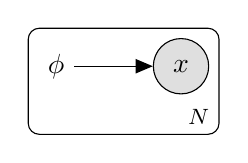
\begin{tikzpicture}
\node[obs] (x) {$ x $};
\node[left=of x] (phi) {$ \phi $};

\edge{phi}{x};

\plate {data} {(x)(phi)} {$ N $};
\end{tikzpicture}
}
\end{column}
\begin{column}{0.6\textwidth}
\alert{(Conditional) Density estimation}
\end{column}

\end{columns}

\begin{tabular}{p{2cm} p{4cm} p{4cm}}
 & Side information ($\phi$) & Observation ($x$) \\ \cline{2-3}
Parsing &   \textcolor{black}{a sentence} & \textcolor{blue}{parse tree} \\
&&\\
Translation &  \textcolor{black}{a sentence in French} & \textcolor{blue}{translation in English} \\
&&\\
Captioning &  \textcolor{black}{an image} & \textcolor{blue}{caption in English} \\
&&\\
Entailment  & \textcolor{black}{a text and hypothesis} & \textcolor{blue}{entailment relation}
\end{tabular}
\end{small}

\end{frame}

\begin{frame}{Where does deep learning kick in?}

Let $\phi$ be all side information available\\
~ e.g. deterministic \emph{inputs/features}

~ \pause

Have neural networks predict parameters of our probabilistic model
	\begin{align*}
    X|\phi \sim \Cat(\pi_{\alert \theta}(\phi)) & & \text{or} & & X|\phi \sim \mathcal N(\mu_{\alert \theta}(\phi), \sigma_{\alert \theta}(\phi)^2)
    \end{align*} \pause
~ and proceed to \alert{estimate parameters} $\theta$ of the NNs %via MLE % that assign maximum likelihood to observations

 





\end{frame}


\begin{comment}
\begin{frame}{Task-driven feature extraction}

Often our side information $\phi$ is itself some high dimensional data
\begin{itemize}
	\item $\phi$ is a sentence and $x$ a tree
	\item $\phi$ is the source sentence and $x$ is the target
	\item $\phi$ is an image and $x$ is a caption
\end{itemize}
and part of the job of the NNs that parametrise our models is to also \alert{deterministically} encode that input in a low-dimensional space

\end{frame}
\end{comment}


\begin{frame}{NN as efficient parametrisation}

From the statistical point of view NNs do not generate data\\
\begin{itemize}
	\item \alert{they parametrise distributions} that \\
	\emph{by assumption} govern data
	\item compact and efficient way to \alert{map from complex side information to parameter space}
\end{itemize}

\vspace{10pt}

\pause
Prediction is done by a decision rule outside the statistical model
\begin{itemize}
	\item e.g. beam search
\end{itemize}

\end{frame}

\begin{frame}{Maximum likelihood estimation}

Let $p(x|\theta)$ be the probability of an observation $x$\\
~and $\theta$ refer to all of its parameters \\
~e.g. parameters of NNs involved

~ \pause

Given a dataset $x^{(1)}, \ldots, x^{(N)}$ of i.i.d. observations, the likelihood function 
\begin{equation*}
\begin{aligned}
\mathcal L(\theta|x^{(1:N)}) &= \log \prod_{s=1}^N p(x^{(s)}|\theta) \\ \pause
 &= \sum_{s=1}^N \log p(x^{(s)}|\theta)
\end{aligned}
\end{equation*} \pause
quantifies the fitness of our model to data

\end{frame}

\begin{frame}{MLE via gradient-based optimisation}

If assessing the log-likelihood is {\bf differentiable} and assessing it is {\bf tractable}, then backpropagation can give us the gradient
\begin{equation*}
\begin{aligned}
\grad_\theta \mathcal L(\theta|x^{(1:N)}) &= \grad_\theta \sum_{s=1}^N \log p(x^{(s)}|\theta) \\ \pause
 &=  \sum_{s=1}^N \grad_\theta \log p(x^{(s)}|\theta)
\end{aligned}
\end{equation*}  \pause

and we can update $\theta$ in the direction
\begin{equation*}
\gamma \grad_\theta \mathcal L(\theta|x^{(1:N)})
\end{equation*}
to attain a local optimum of the likelihood function

\end{frame}

\begin{frame}[plain]{Stochastic optimisation}

We can also use a gradient estimate 
\begin{equation*}
\begin{aligned}
\grad_\theta \mathcal L(\theta|x^{(1:N)}) &= \grad_\theta \underbrace{\mathbb E_{S\sim \mathcal U(1..N)}\left[ N \log p(x^{(S)}|\theta)\right]}_{\mathcal L(\theta|x^{(1:N)})} \\ \pause
 &=  \underbrace{\mathbb E_{S\sim \mathcal U(1..N)}\left[ N \grad_\theta  \log p(x^{(S)}|\theta)\right]}_{\text{expected gradient :)}} \\ \pause
 &\overset{\text{MC}}{\approx} \frac{1}{M} \sum_{m=1}^M N  \grad_\theta \log p(x^{(s_i)}|\theta) \\
 &S_i \sim \mathcal U(1..N)
\end{aligned}
\end{equation*}  \pause
and take steps in the direction
\begin{equation*}
\gamma \frac{N}{M} \grad_\theta \mathcal L(\theta|x^{(s_1:s_M)})
\end{equation*}
where $x^{(s_1)}, \ldots, x^{(s_M)}$ is a random mini-batch of size $M$


\end{frame}



\begin{frame}{DL in NLP recipe}


%Vast majority of papers published at ACL

%\begin{small}
%\begin{figure}
%\scalebox{0.8}{
%\begin{tikzpicture}
%\node[obs] (x) {$ x $};
%\node[left=of x] (phi) {$ \phi $};
%\factor[left=of x] {f} {below:$f_w$} {phi} {x} ; 
%%\edge{phi}{x} ;
%\plate {data} {(x)(phi)} {$ N $};
%\end{tikzpicture}
%}
%\end{figure}
%\end{small}
	Maximum likelihood estimation
	\begin{itemize}
		\item  tells you which \alert{loss} to optimise \\
		(i.e. negative log-likelihood)
	\end{itemize}
	
	\pause
	Automatic differentiation (\emph{backprop})
	\begin{itemize}
		\item chain rule of derivatives: ``give me a tractable forward pass and I will give you \alert{gradients}''
	\end{itemize}
	
	\pause
	Stochastic optimisation powered by backprop
	\begin{itemize}
		\item general purpose gradient-based optimisers
	\end{itemize}

\end{frame}


\begin{frame}{Tractability is central}

Likelihood gives us a differentiable objective to optimise for
\begin{itemize}
	\item but we need to stick with \alert{tractable} likelihood functions
\end{itemize}



%, any intractable likelihood will leave us in bad territory because
%\begin{itemize}
%	\item stochastic optimisation requires gradient estimates
%	\item which must be unbiased (forget greedy techniques)
%	\item and some estimation techniques are not differentiable (forget MC sampling)
%\end{itemize}

\end{frame}

\begin{frame}{When do we have intractable likelihood?}

{\bf Unsupervised problems} contain unobserved random variables\\ 
\begin{equation*}
p_\theta(x, z) = \overbrace{p(z)}^{\text{latent variable model}} \underbrace{p_\theta(x|z)}_{\text{observation model}}
\end{equation*}

~ \pause

thus assessing the marginal likelihood requires \alert{marginalisation of latent variables} 
\begin{equation*}
p_\theta(x) = \int p_\theta(x, z) \dd{z} = \int p(z)p_\theta(x|z) \dd{z} 
\end{equation*}


\end{frame}

\begin{frame}{Examples of latent variable models}

Discrete latent variable, continuous observation
\begin{itemize}
	\item too many forward passes
	\begin{small}
	\begin{equation*}
	p_\theta(x) = \sum_{c=1}^K \Cat(c|\pi_1, \ldots, \pi_K) \underbrace{\mathcal N(x|\mu_\theta(c), \sigma_\theta(c)^2)}_{\text{forward pass}}
	\end{equation*}
	\end{small}
\end{itemize}
	\pause
	
Continuous latent variable, discrete observation
\begin{itemize}
	\item infinitely many forward passes
	\begin{small}
	\begin{equation*}
	p_\theta(x) = \int \mathcal N(z|0, I) \underbrace{\Cat(x|\pi_\theta(z))}_{\text{forward pass}} \mathrm{d}z
	\end{equation*}
	\end{small}
\end{itemize}

\end{frame}

\begin{frame}{Deep generative models}

Joint distribution with {\bf deep observation model}
\begin{equation*}
p_\theta(x, z) = \underbrace{p(z)}_{\text{prior}} \underbrace{p_\theta(x|z)}_{\text{likelihood}}
\end{equation*}
~ {\small mapping from latent variable $z$ to $p(x|z)$ is a NN with parameters $\theta$}

~ \pause

Marginal likelihood (or evidence)
\begin{equation*}
p_\theta(x) = \int p_\theta(x, z) \dd{z} = \int p(z)p_\theta(x|z) \dd{z} 
\end{equation*}
~ \alert{intractable} in general



\end{frame}

\begin{frame}[plain]{Gradient}

Exact gradient is intractable
\begin{small}
\begin{equation*}
\begin{aligned}
\grad_\theta \log p_\theta(x) \pause &= \grad_\theta \log \underbrace{\int p_\theta(x, z) \dd{z}}_{\text{marginal}} \\ \pause
&= \underbrace{\frac{1}{\int p_\theta(x, z) \dd{z}} \int \grad_\theta p_\theta(x,z) \dd{z}}_{\text{chain rule}} \\ \pause
&= \frac{1}{p_\theta(x)} \int \underbrace{p_\theta(x,z) \grad_\theta \log p_\theta(x,z)}_{\text{log-identity for derivatives}} \dd{z} \\ \pause
&= \int \underbrace{\frac{p_\theta(x,z)}{p_\theta(x)}}_{\text{posterior}} \grad_\theta \log p_\theta(x,z) \dd{z} \\ \pause
&= \int p_\theta(z|x) \grad_\theta \log p_\theta(x,z) \dd{z} \\ \pause
&= \underbrace{\mathbb E_{p_\theta(z|x)} \left[ \grad_\theta \log p_\theta(x,Z) \right]}_{\text{expected gradient :)}}
\end{aligned}
\end{equation*}
\end{small}



\end{frame}

\begin{frame}{Can we get an estimate?}

\begin{equation*}
\begin{aligned}
\grad_\theta \log p_\theta(x) 
 &= \mathbb E_{p_\theta(z|x)} \left[ \grad_\theta \log p_\theta(x,Z) \right] \\ \pause
 &\overset{\text{MC}}{\approx} \frac{1}{K} \sum_{k=1}^K \grad_\theta \log p_\theta(x,z^{(k)})  \\
 & z^{(k)} \sim p_\theta(Z|x)
\end{aligned}
\end{equation*}


 \pause

MC estimate of gradient requires sampling from posterior
\begin{small}
\begin{equation*}
p_\theta(z|x) = \frac{p(z)p_\theta(x|z)}{\alert{p_\theta(x)}}
\end{equation*}
\end{small}
~ unavailable due to the intractability of the marginal

\end{frame}


\begin{frame}{Summary}

\begin{itemize}
	\item We like probabilistic models because can make explicit modelling assumptions \pause
	\item We want complex observation models 
	parameterised by NNs \pause
	\item But we cannot use backprop for parameter estimation 
\end{itemize}

\pause

We need \alert{approximate inference} techniques!

\end{frame}

\section{Variational inference}

\begin{frame}{The Basic Problem}
The marginal likelihood
$$ p(x) = \intl{ p(x,z) }{z} $$
is generally \textbf{intractable},  which prevents us from computing quantities that depend on the posterior $p(z|x)$

\begin{itemize}
	\item e.g. gradients in MLE
	\item e.g. predictive distribution in Bayesian modelling
\end{itemize}

\end{frame}


\begin{frame}{Strategy}
Accept that $ p(z|x) $ is not computable.
\pause
\begin{itemize}
	\item approximate it by an auxiliary distribution $ q(z|x) $ that is computable
	\item choose $ q(z|x) $ as close as possible to $ p(z|x) $ to obtain a faithful approximation
\end{itemize}

\end{frame}



\begin{frame}{Evidence lowerbound}

\begin{small}
\begin{equation*}
\begin{aligned}
\log p(x) &= \log \intl{p(x,z)}{z} \\
\pause
&= \log \intl{\alert{q(z|x)}\frac{p(x,z)}{\alert{q(z|x)}}}{z} \\
\pause
&= \loga{\E[q(z|x)]{\frac{p(x,Z)}{{q(Z|x)}}}} \\ \pause
&\geq \underbrace{\E[q(z|x)]{  \log{\frac{p(x,Z)}{{q(Z|x)}}}}}_{\text{ELBO}} \\
\pause
&= \E[q(z|x)]{ \log p(x, Z)} - \E[q(z|x)]{\log q(Z)}\\
\pause
& = \E[q(z|x)] {\log p(x, Z)} + \Ent{q(z|x)}
\end{aligned}
\end{equation*}
\end{small}
\end{frame}

\begin{frame}{An approximate posterior}
\begin{equation*}
\begin{aligned}
\log p(x) &\geq 
\underbrace{\E[q(z|x)] {\log{\frac{p(x, Z)}{q(Z|x)}}}}_{\text{ELBO}} \\
\pause
&= \E[q(z|x)] {\log{\frac{p(Z|x)p(x)}{q(Z|x)}}} \\
\pause
&= \E[q(z|x)] {\log{\frac{p(Z|x)}{q(Z|x)}}} + \underbrace{\log p(x)}_{\text{constant}}\\
\pause
&= - \underbrace{\E[q(z|x)] {\log{\frac{q(Z|x)}{p(Z|x)}}}}_{\KL{q(z|x)}{p(z|x)}} + \log p(x) 
%&= \intl{ q(z|x) \log{\frac{p(Z|x)}{q(Z|x)}}}{z} + \underbrace{\log p(x)}_{\text{constant }} \\ \pause
%&= -\KL{q(z|x)}{p(z|x)} + \log p(x)
\end{aligned}
\end{equation*}
\pause
We have derived a lower bound on the log-evidence whose gap is exactly $ \KL{q(z|x)}{p(z|x)} $.
\end{frame}


\begin{frame}{Variational Inference}
Objective
\begin{equation*}
\underset{q(z|x)}{\max}~\E{\log p(x,Z)} + \Ent{q(z|x)}
\end{equation*}

\begin{itemize}
\item The ELBO is a lower bound on $ \log p(x) $
\end{itemize}

\ack{\citet{BleiEtAl:2016}}
\end{frame}


\begin{frame}{Mean field assumption}

Suppose we have $N$ latent variables\\
\begin{itemize}
	\item assume the posterior factorises as $N$ independent terms
	\item each with an independent set of parameters
\end{itemize}


\begin{equation*}
q(z_1, \ldots, z_N) = \underbrace{\prod_{i=1}^N q_{\lambda_i}(z_i)}_{\text{mean field}}
\end{equation*}


\end{frame}

\begin{frame}{Amortised variational inference}

Amortise the cost of inference using NNs
\begin{equation*}
q(z_1, \ldots, z_N|x_1, \ldots, x_N) = \prod_{i=1}^N q_\lambda(z_i|x_i)
\end{equation*}
~ with a shared set of parameters\\
\begin{itemize}
	\item e.g. $Z|x \sim \mathcal N(\underbrace{\mu_\lambda(x), \sigma_\lambda(x)^2}_{\text{inference network}})$ 
\end{itemize}

\end{frame}


\section{Variational auto-encoder}


\begin{frame}{Variational auto-encoder}

Generative model with NN likelihood

~

\begin{columns}
	\begin{column}{0.2\textwidth}
	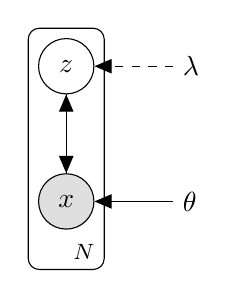
\begin{tikzpicture}
    % Define nodes
    \node[latent]		(z)		{$ z $};
    \node[obs, below = of z]		(x)		{$ x $};
    \node[right = of x]		(theta)		{$ \theta $};
    
    % Connect nodes
    \edge{z,theta}{x};
    
    % add plates
    \plate {x-sentence} {(x)(z)} {$ N $};
   
    \node[right = of z]		(lambda)		{$ \lambda $};   
    \edge[dashed, bend right]{x}{z};
    \edge[dashed]{lambda}{z};
    \end{tikzpicture}
    \end{column}
    \begin{column}{0.7\textwidth}
    	\begin{itemize}
			\item complex (non-linear) observation model $p_\theta(x|z)$
			\item complex (non-linear) mapping from data to latent variables $q_\lambda(z|x)$
    	\end{itemize}
    \end{column}
    \end{columns}
    ~
    
    Jointly optimise generative model $p_\theta(x|z)$ and inference model $q_\lambda(z|x)$ under the same objective (ELBO)
    
    \ack{\citet{KingmaWelling:2013}}
\end{frame}


\begin{frame}[plain]{Objective}

\begin{equation*}
\begin{aligned}
\log p_\theta(x) &\geq \overbrace{\E[q_\lambda(z|x)]{\log p_\theta(x,Z)} + \Ent{q_\lambda(z|x)}}^{\ELBO} \\ 
\pause
&= \E[q_\lambda(z|x)]{\log p_\theta(x|Z) + \log p(Z)} + \Ent{q_\lambda(z|x)} \\ \pause
&= \E[q_\lambda(z|x)]{\log p_\theta(x|Z)} - \KL{q_\lambda(z|x)}{p(z)}
\end{aligned}
\end{equation*}

\pause

Parameter estimation
\begin{equation*}
\argmax_{\theta,\lambda} ~ \E[q_\lambda(z|x)]{\log p_\theta(x|Z)} - \KL{q_\lambda(z|x)}{p(z)}
\end{equation*}

\pause

\begin{itemize}
	\item assume $\KL{q_\lambda(z|x)}{p(z)}$  analytical\\
	true for exponential families \pause
	\item approximate $\E[q_\lambda(z|x)]{\log p_\theta(x|z)}$ by sampling\\
	true because we design $q_\lambda(z|x)$ to be simple
\end{itemize}


\end{frame}

\begin{frame}[plain]{Generative Network Gradient}
\begin{equation*}
\begin{aligned}
&\pdv{\theta} \left( \E[q_\lambda(z|x)]{\log p_\theta(x|z)} - \overbrace{\KL{q_\lambda(z|x)}{p(z)}}^{\text{constant wrt }\theta} \right) \\ \pause 
&=\underbrace{\E[q_\lambda(z|x)]{\pdv{\theta}\log p_\theta(x|z)}}_{\text{expected gradient :)}} \\ \pause
&\overset{\text{MC}}{\approx} \frac{1}{K}\sum_{k=1}^{K}
\pdv{\theta} \log p_\theta(x|z^{(k)}) \\
&z^{(k)} \sim q_\lambda(Z|x)
\end{aligned}
\end{equation*}
\pause
\center{Note: $ q_\lambda(z|x) $ does not depend on $ \theta $.}
\end{frame}

\begin{frame}{Inference Network Gradient}
\begin{equation*}
\begin{aligned}
&\pdv{\lambda}\left(\E[q_\lambda(z|x)]{\log p_\theta(x|z)} - \overbrace{\KL{q_\lambda(z|x)}{p(z)}}^{\text{analytical}} \right) \\ \pause
=&\pdv{\lambda}\E[q_\lambda(z|x)]{\log p_\theta(x|z)} - \underbrace{\pdv{\lambda}\KL{q_\lambda(z|x)}{p(z)}}_{\text{analytical computation}} \\
\end{aligned}
\end{equation*}
\pause
The first term again requires approximation by sampling, \\
~ but there is a problem

\end{frame}

\begin{frame}{Inference Network Gradient}
\begin{equation*}
\begin{aligned}
&\pdv{\lambda}\E[q_\lambda(z|x)]{\log p_\theta(x|z)} \\ \pause
&= \pdv{\lambda} \intl{q_\lambda(z|x)\log p_\theta(x|z)}{z} \\ \pause
&=  \underbrace{\int \alert{\pdv{\lambda}(q_\lambda(z|x))}\log p_\theta(x|z) \dd{z}}_{\text{not an expectation}} 
\end{aligned}
\end{equation*}

\pause

\begin{itemize}
	\item MC estimator is non-differentiable: cannot sample first\\ \pause
	\item Differentiating the expression does not yield an expectation: cannot approximate via MC
\end{itemize}

\end{frame}

\begin{frame}{Score function estimator}

We can again use the log identity for derivatives
\begin{equation*}
\begin{aligned}
&\pdv{\lambda}\E[q_\lambda(z|x)]{\log p_\theta(x|z)} \\ 
&= \pdv{\lambda} \intl{q_\lambda(z|x)\log p_\theta(x|z)}{z} \\ 
&=  \underbrace{\int \alert{\pdv{\lambda}(q_\lambda(z|x))}\log p_\theta(x|z) \dd{z}}_{\text{not an expectation}} \\ \pause
&= \int \textcolor{blue}{q_\lambda(z|x) \pdv{\lambda}(\log q_\lambda(z|x))} \log p_\theta(x|z) \dd{z} \\ \pause
&= \underbrace{\mathbb E_{q_\lambda(z|x)} \left[  \log p_\theta(x|z)  \pdv{\lambda}\log q_\lambda(z|x)\right]}_{\text{expected gradient :)}}
\end{aligned}
\end{equation*}

\end{frame}

\begin{frame}[plain]{Score function estimator: high variance}


We can now build an MC estimator
\begin{equation*}
\begin{aligned}
&\pdv{\lambda}\E[q_\lambda(z|x)]{\log p_\theta(x|z)} \\ 
&= \mathbb E_{q_\lambda(z|x)} \left[  \log p_\theta(x|z)  \pdv{\lambda}\log q_\lambda(z|x)\right] \\ \pause 
&\overset{\text{MC}}{\approx} \frac{1}{K} \sum_{k=1}^K \alert{\log p_\theta(x|z^{(k)})} \pdv{\lambda}\log q_\lambda(z^{(k)}|x) \\
&z^{(k)} \sim q_\lambda(Z|x)
\end{aligned}
\end{equation*}

\pause
but
\begin{itemize}
	\item magnitude of $\log p_\theta(x|z)$ varies widely \pause 
	\item model likelihood does not contribute to direction of gradient \pause
	\item too much variance to be useful
\end{itemize}

\end{frame}

\begin{frame}{When variance is high we can}

\begin{itemize}
	\item sample more \\ \pause
	\alert{won't scale} \pause
	\item use variance reduction techniques (e.g. baselines and control variates)\\ \pause 		\textcolor{orange}{excellent idea, but not just yet} \pause
	\item stare at this $\pdv{\lambda}\E[q_\lambda(z|x)]{\log p_\theta(x|z)}$ \\ \pause
	\textcolor{blue}{until we find a way to rewrite the expectation in terms of a density that 
	{\bf does not depend on} $\lambda$}
\end{itemize}
\end{frame}

\begin{frame}{Reparametrisation}

Find a transformation $ h: z \mapsto \epsilon $ that expresses $z$ through a random variable $\epsilon$ such that \alert{ $q(\epsilon)$ does not depend on $ \lambda $} \pause
\begin{itemize}
\item $ h(z, \lambda) $ needs to be invertible \pause
\item $ h(z, \lambda) $ needs to be differentiable
\pause
\end{itemize}
Invertibility implies
\begin{itemize}
\item $ h(z, \lambda) = \epsilon $
\item $ h^{-1}(\epsilon, \lambda) = z $ 
\end{itemize}

\ack{\citep{KingmaWelling:2013,RezendeEtAl:2014,TitsiasLazarogredilla:2014}}

\end{frame}

\begin{frame}{Gaussian Transformation}

If $Z \sim \mathcal N(\mu_\lambda(x), \sigma_\lambda(x)^2)$ then

\begin{align*}
h(z, \lambda) &= \frac{z - \mu_\lambda(x)}{ \sigma_\lambda(x) } = \epsilon \sim \NDist{0}{\IMatrix} \\
h^{-1}(\epsilon, \lambda) &= \mu_\lambda(x) + \sigma_\lambda(x) \odot \epsilon~~~\epsilon \sim \NDist{0}{\IMatrix}
\end{align*}


\end{frame}

\begin{frame}[plain]{Inference Network -- Reparametrised Gradient}

\begin{equation*}
\begin{aligned}
&= \pdv{\lambda} \int q_\lambda(z|x)\log p_\theta(x|z) \dd{z} \\ \pause
&= \pdv{\lambda} \int \alert{q(\epsilon)} \log p_\theta(x | \alert{\overbrace{h^{-1}(\epsilon, \lambda)}^{=z}}) \dd{\alert{\epsilon}} \\ \pause
&= \int q(\epsilon) \pdv{\lambda} \left[ \log p_\theta(x| \overbrace{h^{-1}(\epsilon, \lambda)}^{=z})\right] \dd{\epsilon} \\ \pause
&= \underbrace{\mathbb E_{q(\epsilon)}\left[ \pdv{\lambda} \log p_\theta(x| h^{-1}(\epsilon, \lambda))\right] \dd{\epsilon}}_{\text{expected gradient :D}} 
%&= \int q(\epsilon) \underbrace{\pdv{z} \log p_\theta(x| h^{-1}(\epsilon, \lambda)) \times \pdv{\lambda} h^{-1}(\epsilon, \lambda)}_{\text{chain rule}} \dd{\epsilon}  \\ \pause
%&= \mathbb E_{q(\epsilon)} \left[ \underbrace{\pdv{z} \log p_\theta(x| \overbrace{h^{-1}(\epsilon, \lambda)}^{=z}) \times \pdv{\lambda} h^{-1}(\epsilon, \lambda)}_{\text{chain rule}} \right]
\end{aligned}
\end{equation*}
\end{frame}

\begin{frame}[plain]{Reparametrised gradient estimate}

\begin{equation*}
\begin{aligned}
&= \underbrace{\mathbb E_{q(\epsilon)}\left[ \pdv{\lambda} \log p_\theta(x| h^{-1}(\epsilon, \lambda))\right] \dd{\epsilon}}_{\text{expected gradient :D}} \\ \pause
&= \mathbb E_{q(\epsilon)} \left[ \underbrace{\pdv{z} \log p_\theta(x| \overbrace{h^{-1}(\epsilon, \lambda)}^{=z}) \times \pdv{\lambda} h^{-1}(\epsilon, \lambda)}_{\text{chain rule}} \right] \\ \pause
&\overset{\text{MC}}{\approx} \frac{1}{K}\sum_{k=1}^{K} \underbrace{\pdv{z} \log p_\theta(x| \overbrace{h^{-1}(\epsilon^{(k)}, \lambda)}^{=z}) \times \pdv{\lambda} h^{-1}(\epsilon^{(k)}, \lambda)}_{\text{backprop's job}}\\
&\epsilon^{(k)} \sim q(\epsilon)
\end{aligned}
\end{equation*}

Note that both models contribute with gradients

\end{frame}

\begin{frame}{Gaussian KL}
\begin{block}{ELBO}
\begin{equation*}
\E[q_\lambda(z|x)]{\log p_\theta(x|z)} - \KL{q_\lambda(z|x)}{p(z)}
\end{equation*}
\end{block}
\pause
Analytical computation of $ -\KL{q_\lambda(z|x)}{p(z)} $:
\begin{equation*}
\frac{1}{2}\sum_{i=1}^{d}\left(1 + \loga{\sigma^{2}_{i}} -
\mu^{2}_{i} - \sigma^{2}_{i} \right)
\end{equation*}
\pause
Thus backprop will compute $-\pdv{\lambda} \KL{q_\lambda(z|x)}{p(z)}$ for us
\end{frame}

\begin{frame}{Computation Graph}
\begin{figure}
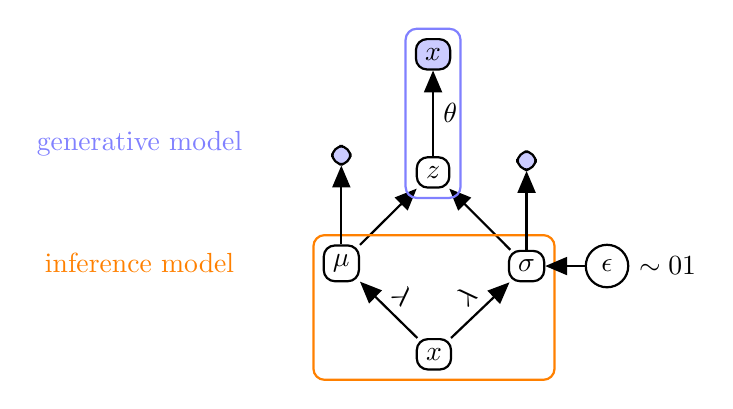
\begin{tikzpicture}[node distance=1cm]
\node[rectangle, draw, rounded corners, thick] (input) {$x$};
\node[rectangle, draw, rounded corners, thick, above left=of input] (mu) {$ \mu $};
\node[rectangle, draw, rounded corners, thick, above right=of input] (var) {$ \sigma $};
\node[rectangle, draw, rounded corners, thick, above right= of mu] (z) {$ z $};
\node[rectangle, fill=blue!20, thick, above of= z, rounded corners, draw, node distance=1.5cm] (output) {$ x $};

\draw[->, thick] (input) -- (mu) node[midway, above, rotate=315] {$ \lambda $};
\draw[->, thick] (input) -- (var) node[midway, above, rotate=45] {$ \lambda $};
\draw[->, thick] (mu) edge (z);
\draw[->, thick] (var) edge (z);
\draw[->, thick] (z) -- (output) node[midway, right] {$ \theta $};

\pause
\node[draw=orange, thick, rectangle, fit= (input) (mu) (var), rounded corners] {};
\node[left= of mu] (inference) {\textcolor{orange}{inference model}};

\pause
\node[draw=blue!50, thick, rectangle, fit= (z) (output), rounded corners] {};
\node[above= of inference] (generation) {\textcolor{blue!50}{generative model}};

\pause
\node[circle, draw, thick ,right =of var, xshift=-.5cm] (epsilon) {$ \epsilon $};
\node[right = of epsilon, xshift=-1cm] (stdNormal) {$ \sim \NDist{0}{1} $};
\draw[->, thick] (epsilon) edge (var);

\pause
\node[above= of mu, rectangle, fill=blue!20, thick, rounded corners, draw,] (KLmu) {$ \KullbackLeibler $};
\draw[->, thick] (mu) edge (KLmu);
\node[above= of var, rectangle, fill=blue!20, thick, rounded corners, draw,] (KLvar) {$ \KullbackLeibler $};
\draw[->, thick] (var) edge (KLvar);
\end{tikzpicture}
\end{figure}
\end{frame}

\begin{frame}{Example}
	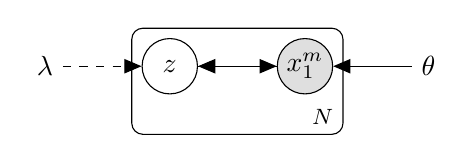
\begin{tikzpicture}
    % Define nodes
    \node[latent]		(z)		{$ z $};
    \node[obs, right = of z]		(x)		{$ x_1^m $};
    \node[right = of x]		(theta)		{$ \theta $};
    
    % Connect nodes
    \edge{z,theta}{x};
    
    % add plates
    \plate {x-sentence} {(x)(z)} {$ N $};
   
    \node[left = of z]		(lambda)		{$ \lambda $};   
    \edge[dashed, bend right]{x}{z};
    \edge[dashed]{lambda}{z};
    \end{tikzpicture}

	Generative model
    	\begin{itemize}
			\item $Z \sim \mathcal N(0, I)$
			\item $X_i | z, x_{<i} \sim \Cat(f_\theta(z, x_{<i}))$\\
			%where $x_{<i}$ is represented by a recurrent hidden state\\
			%and the categorical parameters are predicted by a single hidden layer FFNN with softmax activation
    	\end{itemize}
	Inference model
    	\begin{itemize}
			\item $Z \sim \mathcal N(\mu_\lambda(x_1^m), \sigma_\lambda(x_1^m)^2)$
			%where $x_1^m$ is represented by the average embedding\\
			%location and scale are single hidden layer FFNNs
    	\end{itemize}
	
	
	\ack{\citet{bowman-EtAl:2016}}
	
\end{frame}



\begin{frame}{VAEs -- Summary}
\textbf{Advantages}
\begin{itemize}
\item Backprop training
\item Easy to implement
\item Posterior inference possible
\item One objective for both NNs
\end{itemize}
\pause
\textbf{Drawbacks}
\begin{itemize}
\item Discrete latent variables are difficult
\item Optimisation may be difficult with several latent variables
\item Location-scale families only\\
but see \citet{RuizEtAl:2016} and \citet{KucukelbirEtAl:2017}
\end{itemize}
\end{frame}

%\include{applications}

\begin{frame}{Summary}

Deep learning in NLP
\begin{itemize}
	\item task-driven feature extraction
	\item models with more realistic assumptions
\end{itemize}

~

Probabilistic modelling 
\begin{itemize}
	\item better (or at least more explicit) statistical assumptions
	\item compact models
	\item semi-supervised learning
\end{itemize}


\end{frame}

\begin{frame}[allowframebreaks]{Literature}
\bibliographystyle{plainnat}
\small
\bibliography{VI}
%\nocite{KingmaWelling:2013}
%\nocite{HintonEtAl:1995}
%\nocite{RezendeEtAl:2014}
%\nocite{TitsiasLazarogredilla:2014}
%\nocite{BergkirkpatrickEtAl:2010}
%\nocite{KucukelbirEtAl:2017}
\end{frame}



\end{document}
\grid